%****************************************************************************%
%* DIET User's Manual installing chapter file                               *%
%*                                                                          *%
%*  Author(s):                                                              *%
%*    - Eddy CARON (Eddy.Caron@ens-lyon.fr)                                 *%
%*    - Pushpinder Kaur Chouhan (Pushpinder.Kaur.Chouhan@ens-lyon.fr)       *%
%*    - Philippe COMBES (Philippe.Combes@ens-lyon.fr)                       *%
%*                                                                          *%
%* $LICENSE$                                                                *%
%****************************************************************************%
%* $Id$
%* $Log$
%* Revision 1.14  2008/07/17 21:54:32  ecaron
%* Update scale for figures
%*
%* Revision 1.13  2008/07/17 21:31:46  ecaron
%* To be compliant to latextohtml (use scale instead of resizebox)
%*
%* Revision 1.12  2008/07/16 23:00:12  ecaron
%* Customize look and feel
%*
%* Revision 1.11  2008/04/07 22:25:38  ecaron
%* Updated files to pdflatex compilation
%*
%* Revision 1.10  2006/12/05 12:38:47  ecaron
%* Minor typo fix
%*
%* Revision 1.9  2006/02/06 23:46:34  rbolze
%* change the name of a figure
%*
%* Revision 1.8  2005/07/13 07:57:26  hdail
%* Correction of reference for GoDIET.
%*
%* Revision 1.7  2005/07/12 21:44:28  hdail
%* - Correcting small problems throughout
%* - Modified deployment chapter to have a real section for deploying via GoDIET
%* - Adding short xml example without the comments to make a figure in GoDIET
%*   section.
%*
%* Revision 1.6  2005/07/12 09:23:37  ecaron
%* Chapter introduction
%*
%* Revision 1.5  2005/06/29 08:39:22  hdail
%* Reworded some phrases and corrected some spelling.
%*
%* Revision 1.4  2005/06/24 09:18:34  hdail
%* Using .ps extensions (as done for JXTAConfig.ps) to avoid automatic removal of
%* .eps figures.
%*
%* Revision 1.3  2005/06/24 09:15:11  rbolze
%* add missing file
%*
%* Revision 1.2  2005/06/23 22:53:36  rbolze
%* First version ...
%*
%* Revision 1.1  2005/06/14 08:04:59  ecaron
%* Dashboard section (Todo: Rapha�l)
%*
%* Revision 1.18  2005/05/29 13:51:22  ycaniou
%* Moved the section concerning FAST from description to a new chapter about FAST
%* and performances prediction.
%* Moved the section about convertors in the FAST chapter.
%* Modified the small introduction in chapter 1.
%* The rest of the changes are purely in the format of .tex files.
%*
%* Revision 1.17  2005/05/20 19:06:01  mjan
%* Short description of how to configure DIET for JuxMem
%*
%* Revision 1.16  2004/10/25 08:59:56  sdahan
%* add the multi-MA documentation
%*
%* Revision 1.15  2004/07/12 08:33:58  rbolze
%* explain how to copy cfgs file in install_dir/etc directory and correct my english
%****************************************************************************%

\chapter{DIET dashboard}
\label{ch:dashboard}

This section discussed monitoring tools that can be used with DIET. 
We are currently working on a tool called DIET Dashboard that will
integrate a variety of external tools to provide a single management
and monitoring environment for DIET.  Currently, however, each of
these tools is available separately.  See
Section~\ref{sec:LogService} for a description of LogService, 
Section~\ref{sec:VizDIET} for a description of VizDIET, and 
Section~\ref{sec:deployGoDIET} for a description of GoDIET.

%====[ Dependencies ]==========================================================
\section{LogService}
\label{sec:LogService}
%DIET use a third part software in order to be able to be monitored.
%We have choose to used LogService as monitoring system.
%LogService is a monitoring system which implement the three-thier model and offers
%a easy way to DIET components to be monitored.
%LogService use CORBA for all communication

The DIET platform can be monitored using a system called LogService. 
%\cite{LogService}.
This monitoring service offers the capability to be aware of information that
you want to relay from the platform.  As shown in
Figure~\ref{fig:DIET_LogService}, LogService is composed of three
modules: \textit{LogComponent}, \textit{LogCentral} and
\textit{LogTool}.

 \begin{figure}[h!]
  \begin{center}
    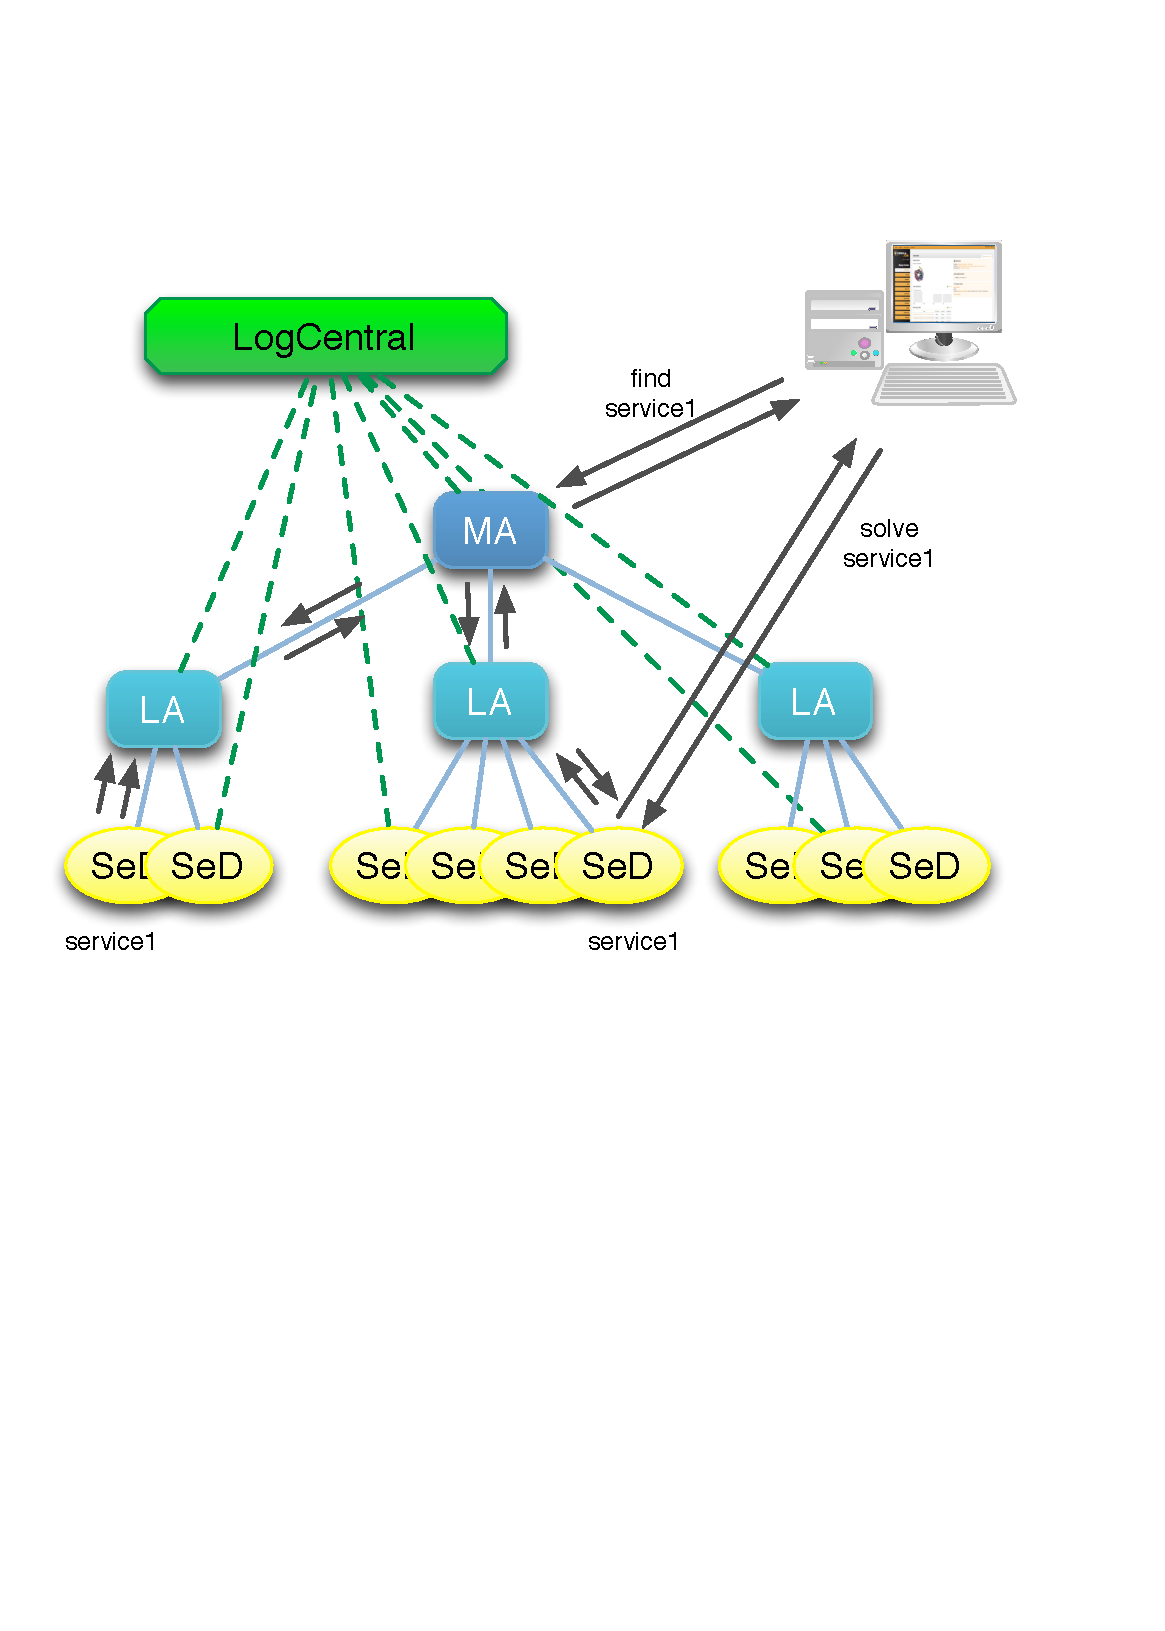
\includegraphics[scale=0.6]{fig/DIET_arch_request-2}
    \caption{DIET and LogService.}
    \label{fig:DIET_LogService}
  \end{center}
\end{figure}

\begin{itemize}
 \item[-] A \textit{LogComponent} is attached to a component and relays
    information and messages to LogCentral.  LogComponents are
    typically used within components one wants to monitor.
 \item[-] \textit{LogCentral} collects messages received from
    \textit{LogComponents}, then \textit{LogCentral} stores or sends
    these messages to \textit{LogTools}.
 \item[-] \textit{LogTools} connect themselves to \textit{LogCentral} and 
    wait for messages.  LogTools are typically used within monitoring tools.
\end{itemize}
The main interest in LogService is that information is collected by
a central point \textit{LogCentral} that receives \textit{logEvents}
from \textit{LogComponents} that are attached to DIET elements (MA,
LA and SeD). \textit{LogCentral} offers the possibility to
re-send this information to several tools (\textit{LogTools})
that are responsible for analysing these message and offering
comprehensive information to the user.\\

\noindent
LogService defines and implements several functionalities:
\begin{description}
  \item[Filtering mechanisms]
    As few messages as possible should be sent to minimize network
    traffic.  With respect to the three-tier model, the
    communications between applications (e.g. LogComponent) and
    the collector (e.g. LogCentral), as well as between the collector
    and the monitoring tools (e.g. LogTools), should be minimized.
    When a LogTool registers with the LogCentral, it also registers
    a filter defining which messages are required by the tool.
  \item[Message ordering]
    Event ordering is another important feature of a monitoring
    system. LogService handles this problem by the introduction of a
    global time line. At generation each message receives a
    time-stamp. The problem that can occur is that the system time
    can be different on each host. LogService measures this
    difference internally and corrects the time-stamps of incoming
    messages accordingly. The time difference is correcting by using
    a time difference measurement recorded during the last ping that
    LogCentral has sent to the LogComponent (pings are sent
    periodically to verify the ``aliveness'' of the LogComponent).

    However, incoming messages are still unsorted. Thus, the
    messages are buffered for a short period of time in order to
    deliver a sorted stream of messages to the tools.  Messages that
    arrive out of order within this time are sorted in the buffer
    and can thus be properly delivered.  Although this induces a
    delivery-delay for messages, this mechanism guarantees the
    proper ordering of messages within a certain tolerance.  As
    tools should not rely on true real-time delivery of messages,
    this short delay is acceptable.
    
  \item[The System State Problem]
    A problem that arises in distributed environments is the state
    of the application. This state may for example contain
    information on connected servers, their relationships, the
    active tasks and many other pieces of information that depend on
    the application.  The system state can be constructed from all
    events that occurred in the application.  Some tools rely on
    this state to work properly.

    The problem emerges if those specific tools do not receive all
    messages.  This might occur as tools can connect to the monitor
    after the application has been started.  In fact, this is quite
    probable as the lifetime of the distributed application can be
    much longer than the lifetime of a tool.

    As a consequence, the system state must be maintained and
    stored.  In order to maintain a system state in a general way,
    LogService does not store the system state itself, but all
    messages which are required to construct it.  Those messages are
    identified by their tag and stored in a special list.  This list
    is forwarded to each tool that connects.  For the tool this
    process is transparent, since it simply receives a number of
    messages that represent the state of the application.
    \label{ref:LogService_system_stats}

    In order to further refine this concept, the list of important
    messages can also be cleaned up by LogService. This is necessary
    as components may connect and disconnect at runtime. After a
    disconnection of a component the respective information is no
    longer relevant for the system state.  Therefore, all messages
    which originated at this component can be removed from the list.
    They have become obsolete due to the disconnection of the
    component and can be safely deleted in order to reduce the
    length of the list of important messages to a minimum.
    \end{description}

All DIET components implement the \textit{LogComponent} interface. By
using LogCentral, the DIET architecture is able to relay information
to LogCentral, and then it is possible to connect to LogCentral by
using a \textit{LogTool} to collect, store and analyse this
information. LogService is available for download. See the web page
\url{http://graal.ens-lyon.fr/DIET/logservice.html} for more
information.

\section{VizDIET}
\label{sec:VizDIET}
VizDIET is the monitoring tool written for DIET to be able to
vizualise and analyse the status and activities of a running DIET
deployment. As described in Section~\ref{sec:LogService},
all DIET's components integrate a \textit{LogComponent}, and VizDIET
implements the \textit{LogTool} interface in order to be able to
collect all information sent by DIET's components through their
\textit{LogComponent}.

VizDIET provides a graphic representation of the DIET architecture
being monitored. There are two ways to use VizDIET.
\begin{description}
        \item[Real-time monitoring:] VizDIET is directly connected
        to the LogCentral using a Corba connection and receives
        directly all information about the running DIET platform.

        \item[Post-mortem monitoring:] VizDIET reads a log file
        containing all log messages received by \textit{LogCentral}.
        This post-mortem analysis can also be replayed in  real time
        if the log file is time sorted.  The log file is created
        during the real deployment by a special tool provided with
        LogService that receives all messages from LogCentral and
        writes them to a file.
\end{description}

\begin{figure}[htb]
  \begin{center}
    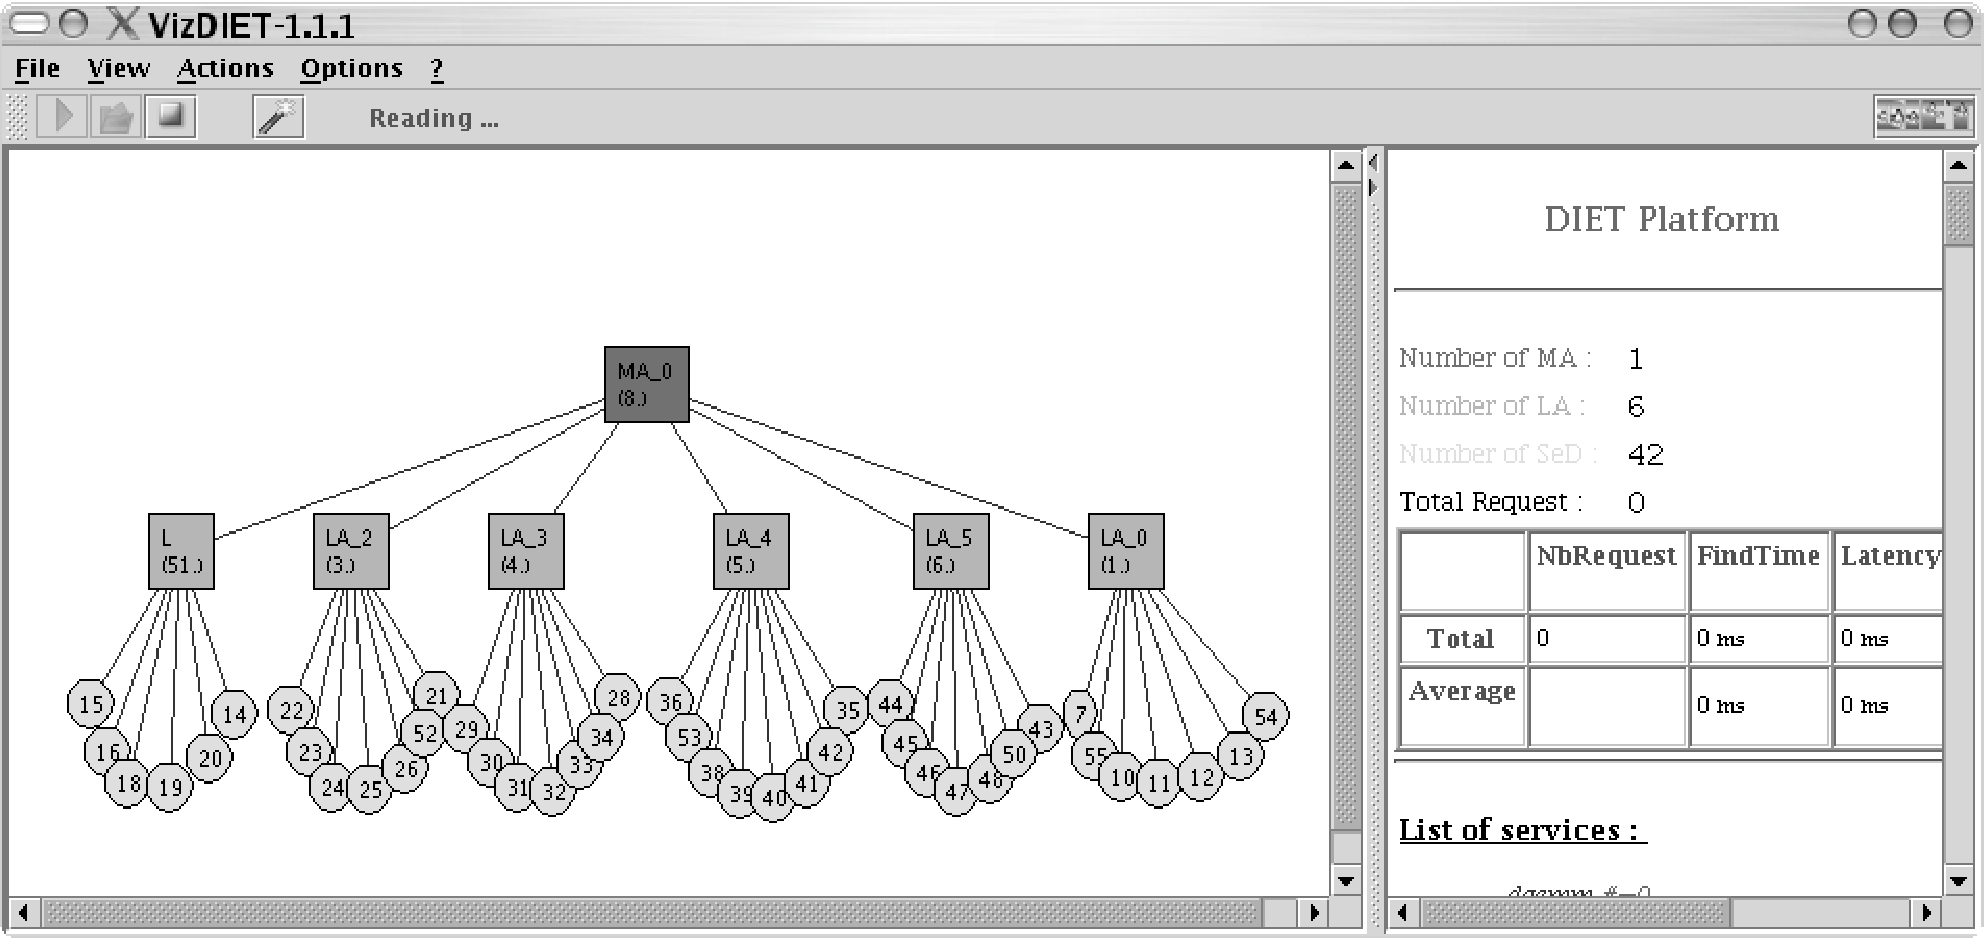
\includegraphics[scale=0.5]{fig/VizDIET}
    \caption{Snapshot of VizDIET.}
    \label{fig:snapshot}
  \end{center}
\end{figure}

As described in Section~\ref{sec:solvepb}, there are two main steps
in the treatment of a request in DIET: one step to find and schedule
a service, and one step to solve this service. So two main
activities are represented: schedule and compute information\\
\begin{description}
  \item [Schedule information]:\\
    When an agent takes a scheduling decision for a task (i.e.
    finding and deciding which SeD can execute a service), it is
    useful to know how the agent made its decision. This information
    is represented by \textit{FindRequest} in VizDIET.
  \item [Compute information]:\\
    When a SeD is computing a job we need to be aware of its state
    and know when the computation begins and ends. This information
    is represented by \textit{SolveRequest}. In VizDIET, when a SeD
    is solving a service, the SeD changes color to red.\\
\end{description}

\begin{figure}[htb]
  \begin{center}
    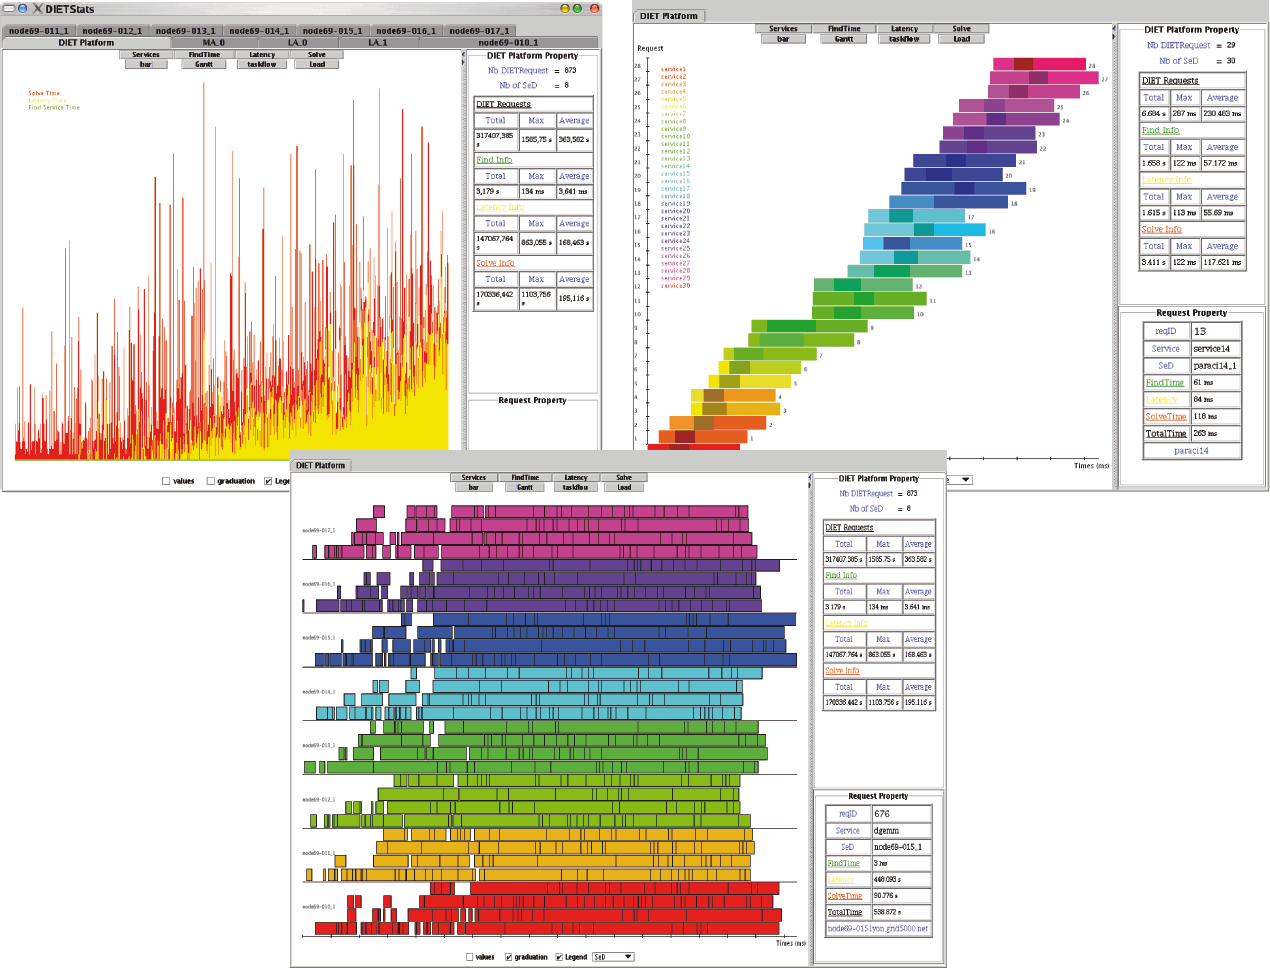
\includegraphics[scale=0.4]{fig/VizDIET_screenshot_2}
    \caption{Bar, taskflow and gantt graphs in vizDIET.}
    \label{fig:vizStats}
  \end{center}
\end{figure}

  \textit{FindRequests} are only attached to agents and
\textit{SolveRequests} are only attached to SeDs. Finally the
aggregation of one \textit{FindRequest} and its
\textit{SolveRequest} is concatenated in one request:
\textit{DIETRequest}. \textit{DIETResquest} can be see as a job
execution in a DIET platform as seen by an end-user. A
\textit{DIETRequest} is also associated with a 
\textbf{latency}, which is time between the end of a
\textit{FindRequest} and the beginning of a \textit{SolveRequest}.

VizDIET offers the possiblity to visualize all of these requests from 
either the point of view of the DIET platform, in which case you
will see the \textit{DIETRequests}, or in the point of view of the
Agents or SeDs, in which case you will see respectively the
\textit{FindRequest} and the \textit{SolveRequest}. The different
kinds of requests are represented in different types of graphics
such as a gantt chart, taskflow chart, or bar chart.

VizDIET also computes some other statistics for the platform such
as average time for scheduling, for solving, or latency. This
information can be see for the whole service in the platform or for
one specific service. VizDIET has one other interesting feature:
the possiblity to export all data collected by VizDIET into
a file using a format that you specify.

Finally, VizDIET is quite useful for understanding the behavior of the
DIET hierarchy and quite simple to use. You have to keep in mind
that VizDIET bases its information upon log information that is
forwarded by LogCentral from DIET components. Therefore, the
information displayed and computed in VizDIET is limited to the DIET
hierarchy (e.g. there is no information about clients).

Future development of VizDIET will depend on new developments in
DIET. For example, a new integration between DIET and JuxMem allows
DIET to store data in the JuxMem service.  Correspondingly, the
capability to log and visualize these transfers has been added to
VizDIET.  VizDIET is available for download. See the web page
\url{http://graal.ens-lyon.fr/DIET/vizdiet.html} for more information.


%\section{Statistic}

